%% Aide-mémoire
\documentclass[10pt, french]{article}
%% -----------------------------
%% Préambule
%% -----------------------------
\usepackage{xcolor}
\usepackage{bbding}
\usepackage{pifont}
\usepackage{tikz}
\usepackage{pgfplots}
\usepackage{array}
\definecolor{LongColor}{HTML}{E61D3B}
\definecolor{ShortColor}{HTML}{2C97D8}
\def\cours{Gestion du risque financier II}
\def\sigle{ACT-2011}
\def\session{Hiver 2018}
\def\auteur{Nicholas Langevin}
\def\BackgroundColor{white}
\def\SectionColor{black!30!black}
\def\SubSectionColor{black!30!black}
\input{cheatsht-preamble.tex}
\title{GRF-II \\ Document d'étude}
\author{Nicholas Langevin}
%% -----------------------------
%% Début du document
%% -----------------------------
\begin{document}

\maketitle 
\vspace{50px}
\begin{center}
\begin{minipage}[c]{7.5cm}
    \begin{itemize}
        \LARGE
        \item[\color{black}\ding{235}] Les produits dérivés 
        \item[\color{black}  \ding{235}] Forwards et autres options
        % \item[\color{purple} \ding{235}] Life Contingencies
        % \item[\color{orange} \ding{235}] Simulation
        % \item[\color{red}    \ding{235}] Statistics
        % \item[\color{blue}   \ding{235}] Extended Linear Model
        % \item[\color{green}  \ding{235}] Time Series      
    \end{itemize}
\end{minipage}
\end{center}
\newpage

\small
\begin{multicols*}{3} % Nombre de colonnes (peut être changé plus tard.)


\section*{Forwards et autres options}
\begin{itemize}[align=left,leftmargin=*]
    \item $\mathbf{T}$: Date d'échéance (\emph{expiration date}).
    \item $\mathbf{r_f}$: Taux d'intérêt sans risque.
    \item $\mathbf{S_0}$: Valeur initiale du sous-jacent (\emph{underlying asset}).
    \item $\mathbf{S_T}$: Valeur à échéance du sous-jacent.
    \item $\mathbf{F_{0,T}}$: Prix à $T$ prédéterminé à $0$ du sous-jacent. $F_{0,T}=S_0(1+r_f)^T$.
    \item $\mathbf{P_0}$: Coût Initial (\emph{premium}). % Notation inventer pour la feuille -> rentre mieux dans les graphiques que: (prime)*(1+r_f)^t
    \item $\mathbf{P_T}$: Coût Initial (\emph{premium}) accumuler à $T$ au taux sans risque. $P_T = P_0(1+r_f)^T$.
    \item \textbf{Payoff}: Valeur à l'échéance.
    \item \textbf{Profil}: Payoff - $P_T$.
    \item {\color{LongColor} \ding{117}} est la couleur d'une position longue.
    \item {\color{ShortColor} \ding{117}} est la couleut d'une position courte.
\end{itemize}
\subsection*{Contrat Forward}
\begin{tabular}{>{\faAngleRight\hspace*{2mm}}lcc}
    \textbf{Position:}& Long & Short \\
    \textbf{Payoff:}& $S_T - F_{0,T}$ & $F_{0,T} - S_T$ \\
    \textbf{Profit:}& $S_T - F_{0,T}$ & $F_{0,T} - S_T$ \\
    \textbf{Max. Loss:}& $F_{0,T}$ & $\infty$ \\
    \textbf{Max. Profit:}& $\infty$ & $F_{0,T}$ \\
\end{tabular}  


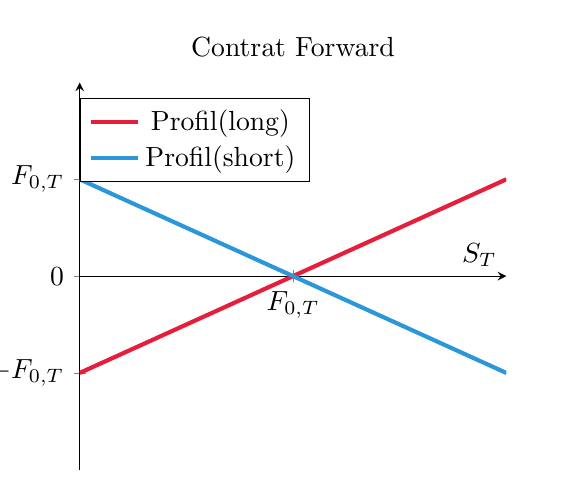
\begin{tikzpicture} % --- CONTRAT FORWARD  ---
    \hspace{-6mm} % Dépend de la grosseur du label de l'axe des y. 
    \begin{axis}[
        height=6.5cm,
        width=7cm,
        axis x line=middle,
        axis y line=left,
        % coordonnées en x
        xlabel={$S_T$},
        xtick={1},
        xticklabels={$F_{0,T}$},
        % Coordonées en y
        ytick={1, 0, -1},
        yticklabels={$F_{0,T}$, 0,$-F_{0,T}$},
        % Légende
        title={Contrat Forward},
        legend entries={Profil(long),Profil(short)},
        legend style={at={(0,0.96)},anchor=north west},
        xmin = 0,
        xmax = 2,
        ymin = -2,
        ymax = 2]
        \addplot[mark=none, draw=LongColor, line width=1.5pt] coordinates { (0,-1) (1,0) (2,1) };
        \addplot[mark=none, draw=ShortColor, line width=1.5pt] coordinates { (0,1) (1,0) (2,-1) };
    \end{axis}
\end{tikzpicture}

\subsection*{Option Call}
\begin{tabular}{>{\faAngleRight\hspace*{2mm}}lc}
    % \hline
    \textbf{Position:}& Long  \\
    \textbf{Coût Initial:} & $-C(K,T)$  \\
    \textbf{Payoff:}& $\max[0,S_T - K]$  \\
    \textbf{Max. Loss:}& $P_T$  \\
    \textbf{Max. Profit:}& $\infty$  \\
    \hline \hline
    \textbf{Position:}& Short  \\
    \textbf{Coût Initial:} & $C(K,T)$  \\
    \textbf{Payoff:}& $-\max[0,S_T - K]$  \\
    \textbf{Max. Loss:}& $\infty$  \\
    \textbf{Max. Profit:}& $P_T$  
\end{tabular}
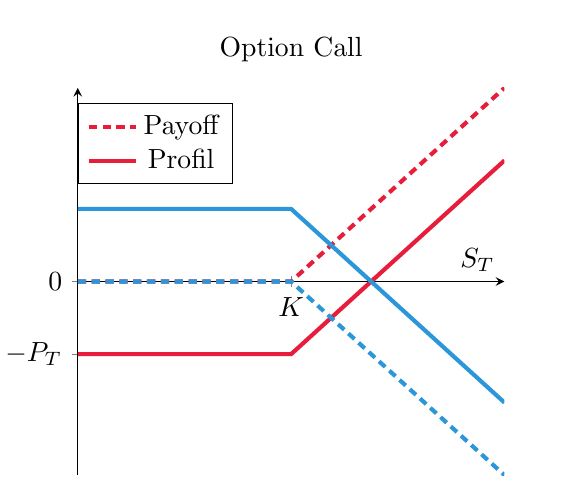
\begin{tikzpicture}
    \hspace{-4mm}
    \begin{axis}[
        height=6.5cm,
        width=7cm,
        axis x line=middle,
        axis y line=left,
        xlabel={$S_T$},
        xtick={1},
        xticklabels={$K$},
        ytick={0, -0.75},
        yticklabels={0,$-P_{T}$},
        title={Option Call},
        legend entries={Payoff,Profil},
        legend style={at={(0,0.96)},anchor=north west},
        xmin = 0,
        xmax = 2,
        ymin = -2,
        ymax = 2]
        \addplot[mark=none, draw=LongColor, line width=1.5pt, densely dashed] coordinates { (0,0) (1,0) (2,2) };
        \addplot[mark=none, draw=LongColor, line width=1.5pt] coordinates { (0,-0.75) (1,-0.75) (2,1.25) };
        \addplot[mark=none, draw=ShortColor, line width=1.5pt, densely dashed] coordinates { (0,0) (1,0) (2,-2) };
        \addplot[mark=none, draw=ShortColor, line width=1.5pt] coordinates { (0,0.75) (1,0.75) (2,-1.25) };
    \end{axis}
\end{tikzpicture}

\subsection*{Option Put}
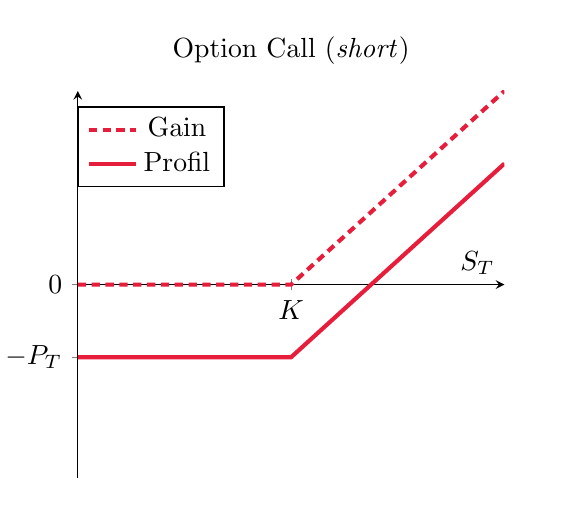
\begin{tikzpicture}
    \hspace{-4mm}
    \begin{axis}[
        height=6.5cm,
        width=7cm,
        axis x line=middle,
        axis y line=left,
        xlabel={$S_T$},
        xtick={1},
        xticklabels={$K$},
        ytick={0, -0.75},
        yticklabels={0,$-P_{T}$},
        title={Option Call (\emph{short})},
        legend entries={Gain,Profil},
        legend style={at={(0,0.96)},anchor=north west},
        xmin = 0,
        xmax = 2,
        ymin = -2,
        ymax = 2]
        \addplot[mark=none, draw=LongColor, line width=1.5pt, densely dashed] coordinates { (0,0) (1,0) (2,2) };
        \addplot[mark=none, draw=LongColor, line width=1.5pt] coordinates { (0,-0.75) (1,-0.75) (2,1.25) };
    \end{axis}
\end{tikzpicture}




\end{multicols*}
%% -----------------------------
%% Fin du document
%% -----------------------------
\end{document}